
%----------------------------------------------------------------------------------------
%	Lecture 19
%----------------------------------------------------------------------------------------

\chapter{Flux and Normal Form of Green's Theorem}

\bigbreak

Flux is another form of line integral.
Let $C$ be plane curve and {\bf F} is a vector field. 
Then, flux is defined as 
$$ \int_C {\bf F} \cdot \hat{n} ds $$

Here, $\hat{n}$ is the unit normal vector to the curve $C$ pointing $90^{\circ}$ clockwise to the direction of the curve.

This is similar to the line integral for work except that in the line integral for work we took the component of the vector field tangent to the curve, that is ${\bf F} \cdot \hat{T}$ where $\hat{T}$ is the unit tangent vector to the curve.
But here we take the component of the vector field normal to the curve.


\section{Physical Interpretation}

For a {\bf F} a velocity field of a fluid, flux measures how much fluid passes passes through $C$ per unit time.

Let's look at what happens on a small portion of our curve.

\begin{figure}[ht!]
    \centering
    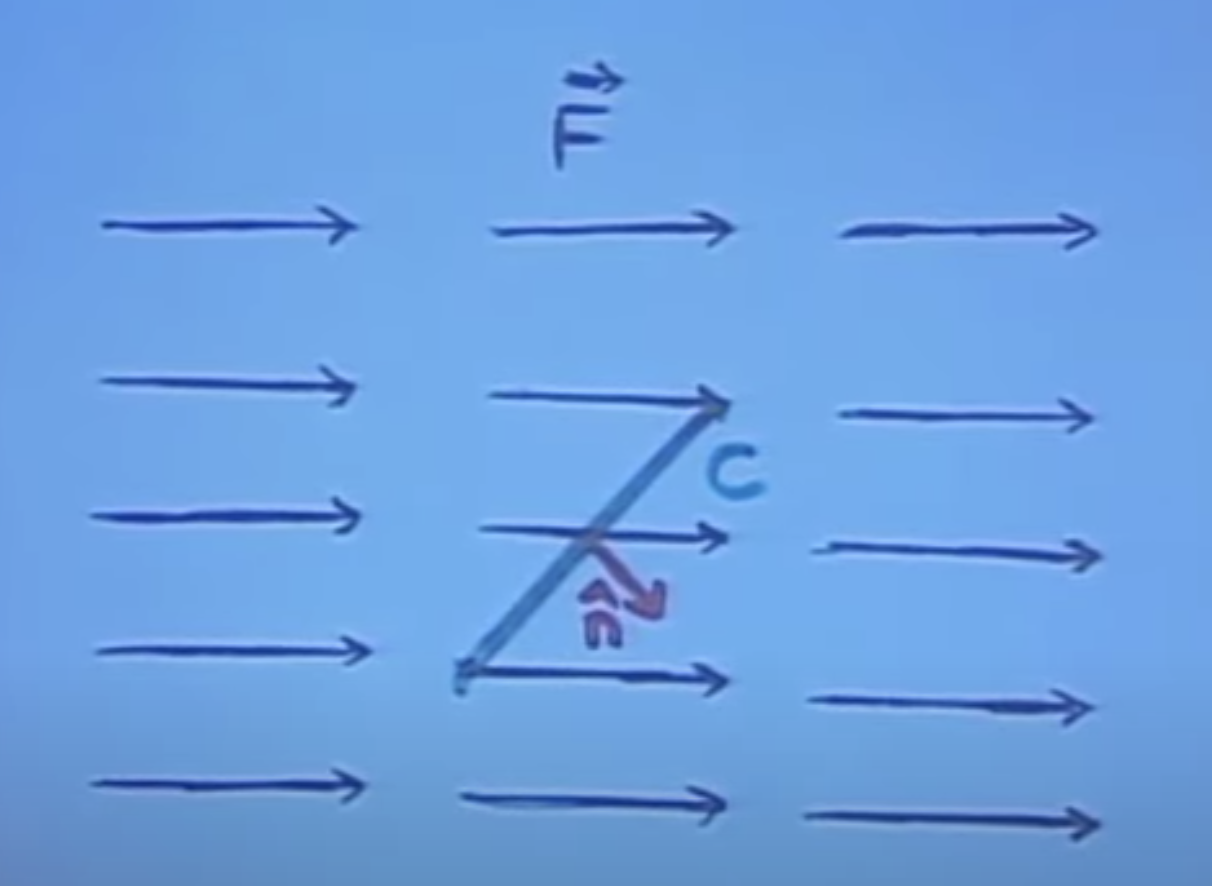
\includegraphics[scale=0.3]{./images/lecture_19_figure_1.png}
    \caption{Smallest portion of a curve}
\end{figure}

Here we are drawing a constant vector field because if zoom enough then the vector field is constant everywhere.
So now how much fluid goes through the curve will be a parallelogram that we show below.

\begin{figure}[ht!]
    \centering
    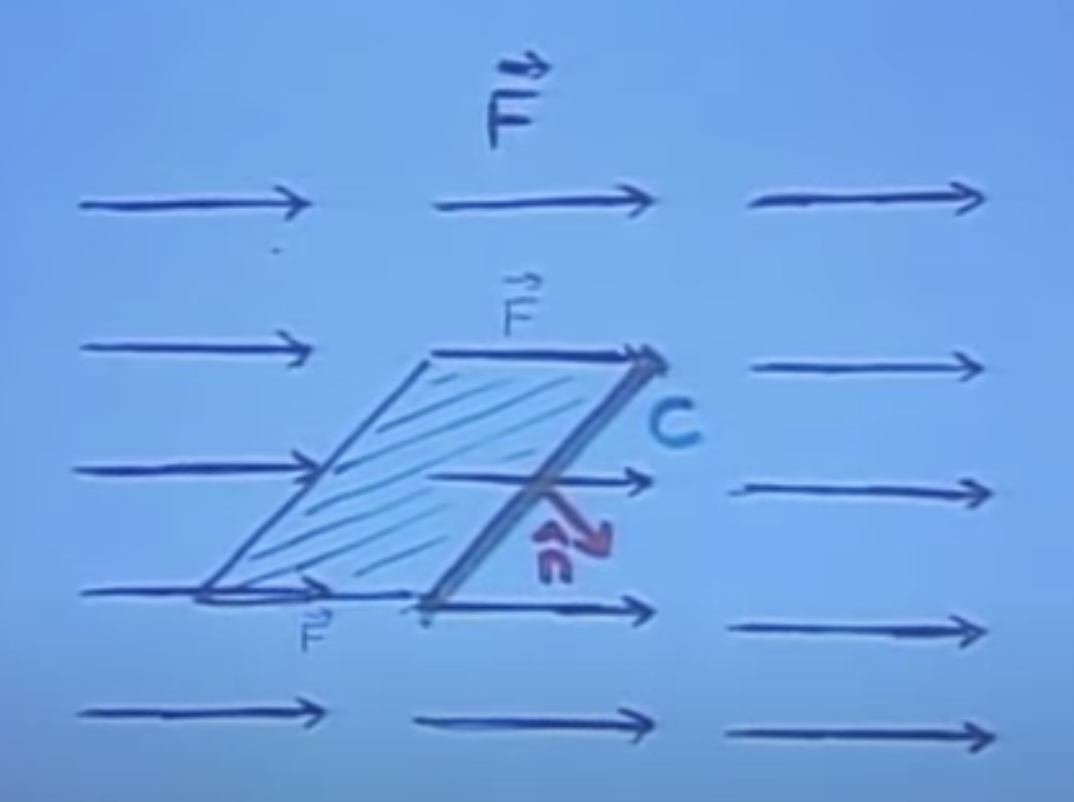
\includegraphics[scale=0.3]{./images/lecture_19_figure_2.png}
    \caption{Amount of fluid going through the curve}
\end{figure}

Now let's try to figure out the area of the parallelogram.
The length of the curve will be $\Delta s$ and the height will be the normal component of ${\bf F}$ which is ${\bf F} \cdot \hat{n}$.
Thus summing the area over the whole curve gets us $\sum {\bf F} \cdot \hat{n} \Delta s$ which is the flux in the limit $\Delta s \to 0$.

\section{Computation of the Flux}

\subsection{Examples}

{\bf Example 1.}  Let's say that $C$ is circle of radius $a$ in counterclockwise direction.
And ${\bf F} = \ij{x}{y}$ which is the radius vector at each point.

When we go counterclockwise direction on a closed curve then the normal vector points to towards the outside of the curve.
So we are measuring the flux going out the curve.

Here the vector field ${\bf F}$ and the normal vector $\hat{n}$ are parallel. So ${\bf F} \cdot \hat{n} = |{\bf F}|$.
Now the magnitude of ${\bf F}$ is $\sqrt(x^2+y^2)$ and each point on the curve this value is equal to $a$.
So our flux is 
$$ Flux = \int_C {\bf F} \cdot \hat{n} ds = \int_C |{\bf F}| ds = \int_C a ds = a * length(C) = a * (2 \pi a) = 2\pi a^2 $$


{\bf Example 2.} Let's say the curve is the same as the last example and ${\bf F} = \ij{-y}{x}$.
Now ${\bf F}$ is tangent to $C$ so ${\bf F} \cdot \hat{n} = 0$ so the flux will be zero.


\subsection{Computing Flux in Coordinates}

Remember $d{\bf r} = \hat{T} ds = \left< dx, dy \right>$.
Now $\hat{n}$ is $\hat{T}$ rotated clockwise by $90^{\circ}$ so $\hat{n} ds = \left< dy, - dx \right>$.
Thus, flux becomes
$$ 
\int_C {\bf F} \cdot \hat{n} ds 
    = \int_C {\bf F} \cdot \left< dy, -dx \right>
    = \int_C Mdy - Ndx
    = \int_C - N dx + M dy
$$

Here, we can parametrize the curve and then convert the flux into a single variable integral.

\pagebreak

\section{Green's Theorem for Flux}

\begin{mdframed}
\begin{center}
If a closed curve $C$ encloses a region $R$ in counterclockwise direction, 
and a vector field ${\bf F} = \left< P, Q \right>$ is defined and differentiable in $R$ then
$$
\oint_C {\bf F} \cdot \hat{n} ds = \iint_R div({\bf F}) dx dy
$$
where $div({\bf F}) = P_x + Q_y$ is called divergence of ${\bf F}$.
\end{center}
\end{mdframed}

This is called Green's Theorem in normal form. 
And the Green's Theorem for Work is said to be in tangential form.

\subsection{Proof of Green's Theorem for Flux}

We know that, 
$$ Flux = \oint_C -Q dx + P dy $$
Let $M = -Q$ and $N = P$ so we get
$$ Flux = \oint_C M dx + N dy $$
But the original Green's Theorem, states that
$$ \oint_C M dx + N dy = \iint_R N_x - M_y dA $$
Thus, applying that we get,
$$ Flux = \iint_R N_x - M_y dA = \iint_R P_x + Q_y dA $$
Thus, 
$$ \oint_C {\bf F} \cdot \hat{n} ds = \oint_C - Q dx + P dy = \iint_R P_x + Q_y dA $$
Hence, proved.

\section{Interpretation Of Divergence}

If you take a vector field which is constant or rotating, then there is no divergence.
Divergence is a measure of expanding motion. That is, it measures how much the flow is expanding.

If the vector field represents the velocity of a fluid then the fluid will take up more and more space if the divergence is positive.
Otherwise it will take less and less space if the divergence is negative as time passes.

The another way to think about it is the amount of fluid being inserted into the system per unit time and per unit area.
